%iffalse
\let\negmedspace\undefined
\let\negthickspace\undefined
\documentclass[journal,12pt,onecolumn]{IEEEtran}
\usepackage{cite}
\usepackage{amsmath,amssymb,amsfonts,amsthm}
\usepackage{algorithmic}
\usepackage{graphicx}
\usepackage{textcomp}
\usepackage{xcolor}
\usepackage{txfonts}
\usepackage{listings}
\usepackage{enumitem}
\usepackage{mathtools}
\usepackage{gensymb}
\usepackage{comment}
\usepackage[breaklinks=true]{hyperref}
\usepackage{tkz-euclide} 
\usepackage{listings}
\usepackage{gvv}                                        
%\def\inputGnumericTable{}                                 
\usepackage[latin1]{inputenc}     
\usepackage{xparse}
\usepackage{color}                                            
\usepackage{array}                                            
\usepackage{longtable}                                       
\usepackage{calc}                                             
\usepackage{multirow}
\usepackage{multicol}
\usepackage{hhline}                                           
\usepackage{ifthen}                                           
\usepackage{lscape}
\usepackage{tabularx}
\usepackage{array}
\usepackage{float}
\newtheorem{theorem}{Theorem}[section]
\newtheorem{problem}{Problem}
\newtheorem{proposition}{Proposition}[section]
\newtheorem{lemma}{Lemma}[section]
\newtheorem{corollary}[theorem]{Corollary}
\newtheorem{example}{Example}[section]
\newtheorem{definition}[problem]{Definition}
\newcommand{\BEQA}{\begin{eqnarray}}
\newcommand{\EEQA}{\end{eqnarray}}
\usepackage{float}
%\newcommand{\define}{\stackrel{\triangle}{=}}
\theoremstyle{remark}
\usepackage{ circuitikz }
%\newtheorem{rem}{Remark}
% Marks the beginning of the document
\begin{document}
\title{CH: Chemical Engineering}
\author{EE25BTECH11012 - BEERAM MADHURI}
\maketitle
\renewcommand{\thefigure}{\theenumi}
\renewcommand{\thetable}{\theenumi}

\begin{enumerate}
\item Which ONE of the following is NOT an integrating factor for the differential equation $x dy - y dx = 0$?
\hfill{\brak{\text{CH 2008}}}
\begin{enumerate}
\begin{multicols}{4}
    \item $\frac{1}{x^2}$
    \item $\frac{1}{y^2}$
    \item $\frac{1}{xy}$
    \item $\frac{1}{(x + y)}$
\end{multicols}
\end{enumerate}

\item Which ONE of the following is NOT a solution of the differential equation $\frac{d^2y}{dx^2} + y = 1$?
\hfill{\brak{\text{CH 2008}}}
\begin{enumerate}
\begin{multicols}{4}
    \item $y = 1$
    \item $y = 1 + \cos x$
    \item $y = 1 + \sin x$
    \item $y = 2 + \sin x + \cos x$
\end{multicols}
\end{enumerate}

\item The limit of $\frac{\sin x}{x}$ as $x \rightarrow \infty$ is
\hfill{\brak{\text{CH 2008}}}
\begin{enumerate}
\begin{multicols}{4}
    \item $-1$
    \item $0$
    \item $1$
    \item $\infty$
\end{multicols}
\end{enumerate}

\item The unit normal vector to the surface of the sphere $x^2 + y^2 + z^2 = 1$ at the point $\left(\frac{1}{\sqrt{2}}, 0, \frac{1}{\sqrt{2}}\right)$ is
\hfill{\brak{\text{CH 2008}}}
\begin{enumerate}
\begin{multicols}{4}
    \item$\frac{1}{\sqrt{2}} \hat{i} + \frac{1}{\sqrt{2}} \hat{j}$
    \item $\frac{1}{\sqrt{2}} \hat{i} + \frac{1}{\sqrt{2}} \hat{k}$
    \item $\frac{1}{\sqrt{2}} \hat{j} + \frac{1}{\sqrt{2}} \hat{k}$
    \item $\frac{1}{\sqrt{3}} \hat{i} + \frac{1}{\sqrt{3}} \hat{j} + \frac{1}{\sqrt{3}} \hat{k}$
\end{multicols}
\end{enumerate}

\item A nonlinear function $f(x)$ is defined in the interval $-1.2 < x < 4$. The equation $f(x) = 0$ is solved for $x$ using the Newton-Raphson iterative scheme. Among the initial guesses ($I_1, I_2, I_3$ and $I_4$), the guess that is likely to lead to the root most rapidly is
\begin{figure}[H]
\centering
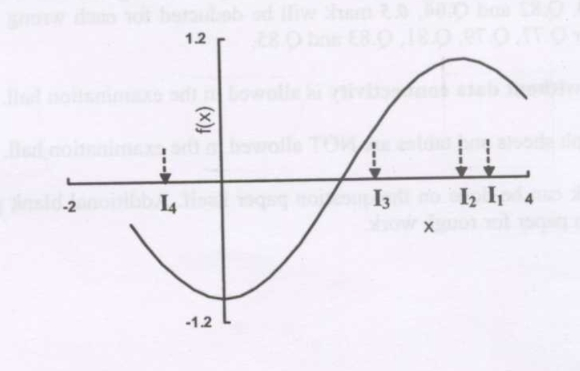
\includegraphics[width=0.25\columnwidth]{figs/qn5.jpg}
\caption{}
\label{fig:qn5.jpg}
\end{figure}
\hfill{\brak{\text{CH 2008}}}
\begin{enumerate}
\begin{multicols}{4}
    \item $I_1$
    \item $I_2$
    \item $I_3$
    \item $I_4$
    \end{multicols}
    \end{enumerate}

\item For a Carnot refrigerator operating between $40^\circ\text{C}$ and $25^\circ\text{C}$, the coefficient of performance is
\hfill{\brak{\text{CH 2008}}}
    \begin{enumerate}[label=(\Alph*)]
    \begin{multicols}{4}
        \item $1$
        \item $1.67$
        \item $19.88$
        \item $39.74$
    \end{multicols}
    \end{enumerate}

\item The work done by one mole of a van der Waals fluid undergoing reversible isothermal expansion from initial volume $V_i$ to final volume $V_f$ is
\hfill{\brak{\text{CH 2008}}}
    \begin{enumerate}[label=(\Alph*)]
    \begin{multicols}{2}
        \item $RT \ln \left( \frac{V_f}{V_i} \right)$
        \item $RT \ln \left( \frac{V_f - b}{V_i - b} \right)$
        \item $RT \ln \left| \frac{V_f - b}{V_i - b} \right| - a \left( \frac{1}{V_f} - \frac{1}{V_i} \right)$
        \item $RT \ln \left( \frac{V_f - b}{V_i - b} \right) + a \left( \frac{1}{V_f} - \frac{1}{V_i} \right)$
    \end{multicols}
    \end{enumerate}

\item For a system containing species P, Q and R, composition at point k on the ternary plot is
    \begin{figure}[H]
    \centering
    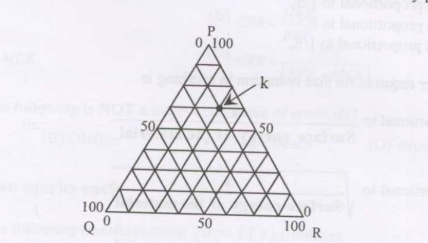
\includegraphics[width=0.25\columnwidth]{figs/qn8.jpg}
    \caption{}
    \label{fig:qn8.jpg}
    \end{figure}
    \hfill{\brak{\text{CH 2008}}}
    \begin{enumerate}[label=(\Alph*)]
    \begin{multicols}{2}
        \item $62.5\%$ P, $12.5\%$ Q, $25\%$ R
        \item $25\%$ P, $62.5\%$ Q, $12.5\%$ R
        \item $12.5\%$ P, $62.5\%$ Q, $25\%$ R
        \item $12.5\%$ P, $25\%$ Q, $62.5\%$ R
    \end{multicols}
    \end{enumerate}

    \item Three containers are filled with water up to the same height as shown. The pressures at the bottom of the containers are denoted as $P_1$, $P_2$ and $P_3$. Which ONE of the following relationships is true?
    \begin{figure}[H]
        \centering
        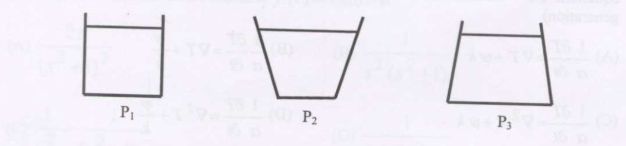
\includegraphics[width=0.5\linewidth]{figs/qn9.jpg}
        \caption{}
        \label{fig:qn9.jpg}
    \end{figure}
    \hfill{\brak{\text{CH 2008}}}
    \begin{enumerate}[label=(\Alph*)]
    \begin{multicols}{4}
        \item $P_1 > P_3 > P_2$
        \item $P_2 > P_1 > P_3$
        \item $P_1 > P_2 = P_3$
        \item $P_1 = P_2 = P_3$
    \end{multicols}
    \end{enumerate}

    \item Losses for flow through valves and fittings are expressed in terms of
    \hfill{\brak{\text{CH 2008}}}
    \begin{enumerate}[label=(\Alph*)]
    \begin{multicols}{2}
        \item drag coefficient
        \item equivalent length of a straight pipe
        \item shape factor
        \item roughness factor
    \end{multicols}
    \end{enumerate}

    \item To determine the performance of a compressor, a standardized test is performed. In the testing process, when the compressor is under operation, ``shut off'' term signifies
    \hfill{\brak{\text{CH 2008}}}
    \begin{enumerate}[label=(\Alph*)]
    \begin{multicols}{2}
        \item maximum flow
        \item zero flow
        \item steady flow
        \item intermittent flow
    \end{multicols}
    \end{enumerate}

    \item Given a pipe of diameter $D$, the entrance length necessary to achieve fully developed laminar flow is proportional to ( $N_{\text{Re}}$ is Reynolds number)
    \hfill{\brak{\text{CH 2008}}}
    \begin{enumerate}[label=(\Alph*)]
    \begin{multicols}{4}
        \item $D \, N_{\text{Re}}$
        \item $\frac{D}{N_{\text{Re}}}$
        \item $D \, N_{\text{Re}}^2$
        \item $\frac{D}{N_{\text{Re}}^2}$
    \end{multicols}
    \end{enumerate}

    \item For laminar flow conditions, the relationship between the pressure drop $(\Delta P_c)$ across an incompressible filter cake and the specific surface area $(S_o)$ of the particles being filtered is given by ONE of the following
    \hfill{\brak{\text{CH 2008}}}
    \begin{enumerate}[label=(\Alph*)]
    \begin{multicols}{2}
        \item $\Delta P_c$ is proportional to $S_o$
        \item $\Delta P_c$ is proportional to $1/S_o$
        \item $\Delta P_c$ is proportional to $S_o^2$
        \item $\Delta P_c$ is proportional to $1/S$
        \end{multicols}
        \end{enumerate}
        
    \item The power required for size reduction in crushing is
    \hfill{\brak{\text{CH 2008}}}
    \begin{enumerate}[label=(\Alph*)]
        \item proportional to $\dfrac{1}{\text{Surface energy of the material}}$
        \item proportional to $\sqrt{\dfrac{1}{\text{Surface energy of the material}}}$
        \item proportional to Surface energy of the material
        \item independent of the Surface energy of the material
    \end{enumerate}

    \item Transient three-dimensional heat conduction is governed by ONE of the following differential equations ($\alpha$ - thermal diffusivity, $k$ - thermal conductivity and $\psi$ - volumetric rate of heat generation)
    \hfill{\brak{\text{CH 2008}}}
    \begin{enumerate}[label=(\Alph*)]
    \begin{multicols}{2}
        \item $\dfrac{1}{\alpha} \dfrac{\partial T}{\partial t} = \nabla T + \psi k$
        \item $\dfrac{1}{\alpha} \dfrac{\partial T}{\partial t} = \nabla T + \dfrac{\psi}{k}$
        \item $\dfrac{1}{\alpha} \dfrac{\partial T}{\partial t} = \nabla^2 T + \psi k$
        \item $\dfrac{1}{\alpha} \dfrac{\partial T}{\partial t} = \nabla^2 T + \dfrac{\psi}{k}$
        \end{multicols}
    \end{enumerate}

    \item In a countercurrent gas absorber, both the operating and equilibrium relations are linear. The inlet liquid composition and the exit gas composition are maintained constant. In order to increase the absorption factor
    \hfill{\brak{\text{CH 2008}}}
    \begin{enumerate}[label=(\Alph*)]
        \item the liquid flow rate should decrease
        \item the gas flow rate should increase
        \item the slope of the equilibrium line should increase
        \item the slope of the equilibrium line should decrease
    \end{enumerate}

    \item A species ($A$) reacts on a solid catalyst to produce $R$ and $S$ as follows:
    \begin{align*}
        A &\rightarrow R \qquad r_R = k_1 C_A^2 \\
        A &\rightarrow S \qquad r_S = k_2 C_A^2
    \end{align*}
    Assume film resistance to mass transfer is negligible. The ratio of instantaneous fractional yield of $R$ in the presence of pore diffusion to that in the absence of pore diffusion is
    \hfill{\brak{\text{CH 2008}}}
    \begin{enumerate}[label=(\Alph*)]
    \begin{multicols}{4}
        \item $1$
        \item $>1$
        \item $<1$
        \item $Zero$
    \end{multicols}
    \end{enumerate}

    \item For the case of single lump-sum capital expenditure of Rs. 10 crores which generates a constant annual cash flow of Rs. 2 crores in each subsequent year, the payback period (in years), if the scrap value of the capital outlay is zero is
    \hfill{\brak{\text{CH 2008}}}
    \begin{enumerate}[label=(\Alph*)]
    \begin{multicols}{4}
        \item $10$
        \item $20$
        \item $1$
        \item $5$
    \end{multicols}
    \end{enumerate}

    \item The relation between capital rate of return ratio (CRR), net present value (NPV) and maximum cumulative expenditure (MCE) is
    \hfill{\brak{\text{CH 2008}}}
    \begin{enumerate}[label=(\Alph*)]
    \begin{multicols}{2}
        \item $CRR = \dfrac{NPV}{MCE}$
        \item $CRR = \dfrac{MCE}{NPV}$
        \item $CRR = NPV \times MCE$
        \item $CRR = \dfrac{MCE}{(NPV + MCE)}$
    \end{multicols}
    \end{enumerate}

    \item Which ONE of the following is NOT a major constituent of crude oil?
    \hfill{\brak{\text{CH 2008}}}
    \begin{enumerate}[label=(\Alph*)]
    \begin{multicols}{4}
        \item Paraffins
        \item Olefins
        \item Naphthenes
        \item Aromatics
    \end{multicols}
    \end{enumerate}

   \item Which ONE of the following transformations $\{ u = f(y) \}$ reduces $\frac{dy}{dx} + Ay^3 + By = 0$ to a linear differential equation? \quad (A and B are positive constants)
   \hfill{\brak{\text{CH 2008}}}
\begin{enumerate}
\begin{multicols}{4}
\item $u = y^{-3}$
\item $u = y^{-2}$
\item $u = y^{-1}$
\item $u = y^2$
\end{multicols}
\end{enumerate}

\item The Laplace transform of the function $f(t) = t \sin t$ is
\hfill{\brak{\text{CH 2008}}}
\begin{enumerate}
\begin{multicols}{2}
\item $\frac{2s}{(s^2+1)^2}$
\item $\frac{1}{s^2(s^2+1)}$
\item $\frac{1}{s^2} + \frac{1}{(s^2+1)}$
\item $\frac{1}{(s-1)^2+1}$
\end{multicols}
\end{enumerate}

\item The value of the surface integral $\iint_S (x\hat{i}+y\hat{j})\cdot\hat{n}\,dA$ evaluated over the surface of a cube having sides of length $a$ is ($\hat{n}$ is unit normal vector)
\hfill{\brak{\text{CH 2008}}}
\begin{enumerate}
\begin{multicols}{4}
\item $0$
\item $a^3$
\item $2a^3$
\item $3a^3$
\end{multicols}
\end{enumerate}

\item The first four terms of the Taylor series expansion of $\cos X$ about the point $x = 0$ are
\hfill{\brak{\text{CH 2008}}}
\begin{enumerate}
\item $1 + x + \frac{x^2}{2!} + \frac{x^3}{3!}$
\item $1 - x + \frac{x^2}{2!} - \frac{x^3}{3!}$
\item $1 - \frac{x^2}{2!} + \frac{x^4}{4!} - \frac{x^6}{6!}$
\item $x - \frac{x^3}{3!} + \frac{x^5}{5!} - \frac{x^7}{7!}$
\end{enumerate}

\item If $A = \begin{bmatrix} 1 & 2 \\ 2 & 1 \end{bmatrix}$, then the eigenvalues of $A^3$ are
\hfill{\brak{\text{CH 2008}}}
\begin{enumerate}
\begin{multicols}{4}
\item $5, 4$
\item $3, -1$
\item $9, -1$
\item $27, -1$
\end{multicols}
\end{enumerate}

\item An analytic function $\mathrm{w}(z)$ is defined as $\mathrm{w}=u+\mathrm{i}v$, where $\mathrm{i} = \sqrt{-1}$ and $z = x + \mathrm{i}y$. If the real part is given by $u=\frac{y}{x^2 + y^2}$, $\mathrm{w}(z)$ is
\hfill{\brak{\text{CH 2008}}}
\begin{enumerate}
\begin{multicols}{4}
\item $\frac{1}{z}$
\item $\frac{1}{z^2}$
\item $\frac{\mathrm{i}}{z}$
\item $\frac{1}{\mathrm{i}z}$
\end{multicols}
\end{enumerate}

\item The normal distribution is given by
\[f(x) = \frac{1}{\sqrt{2\pi} \sigma} \exp \left( -\frac{(x-\mu)^2}{2\sigma^2} \right), \quad -\infty<x<\infty\]
The points of inflexion to the normal curve are
\hfill{\brak{\text{CH 2008}}}
\begin{enumerate}
\begin{multicols}{2}
\item $x = -\sigma, +\sigma$
\item $x = \mu + \sigma, \mu - \sigma$
\item $x = \mu + 2\sigma, \mu - 2\sigma$
\item $x = \mu + 3 \sigma, \mu - 3\sigma$
\end{multicols}
\end{enumerate}

\item Using Simpson's $1/3$ rule and FOUR equally spaced intervals ($n = 4$), estimate the value of the integral $\int_{0}^{\frac{\pi}{4}} \frac{\sin x}{\cos^3 x} \, dx$
\hfill{\brak{\text{CH 2008}}}
\begin{enumerate}
\begin{multicols}{4}
    \item $0.3887$
    \item $0.4384$
    \item $0.5016$
    \item $0.5527$
\end{multicols}
\end{enumerate}

\item The following differential equation is to be solved numerically by the Euler's explicit method.
\[\frac{dy}{dx} = x^2 y - 1.2 y \text{ with } y(0)=1\]
A step size of $0.1$ is used. The solution for $y$ at $x=0.1$ is
\hfill{\brak{\text{CH 2008}}}
\begin{enumerate}
\begin{multicols}{4}
    \item $0.880$
    \item $0.905$
    \item $1.000$
    \item $1.100$
\end{multicols}
\end{enumerate}

\item The Poisson distribution is given by $P(r) = \frac{m^r}{r!} \exp(-m)$. The first moment about the origin for this distribution is
\hfill{\brak{\text{CH 2008}}}
\begin{enumerate}
\begin{multicols}{4}
    \item $0$
    \item $m$
    \item $1/m$
    \item $m^2$
\end{multicols}
\end{enumerate}

\item Air ($79$ mole $\%$ nitrogen and $21$ mole $\%$ oxygen) is passed over a catalyst at high temperature. Oxygen completely reacts with nitrogen as shown below
\hfill{\brak{\text{CH 2008}}}
\[\begin{aligned}    0.5 \mathrm{N}_{2(\mathrm{g})} + 0.5 \mathrm{O}_{2(\mathrm{g})} &\rightarrow \mathrm{NO}_{(\mathrm{g})} \\    0.5 \mathrm{N}_{2(\mathrm{g})} + \mathrm{O}_{2(\mathrm{g})} &\rightarrow \mathrm{NO}_{2(\mathrm{g})}\end{aligned}\]
The molar ratio of $\mathrm{NO}$ to $\mathrm{NO}_2$ in the product stream is $2:1$. The fractional conversion of nitrogen is
\hfill{\brak{\text{CH 2008}}}
\begin{enumerate}
\begin{multicols}{4}
    \item $0.13$
    \item $0.20$
    \item $0.27$
    \item $0.40$
\end{multicols}
\end{enumerate}

\item A $35$ wt$\%$ $\mathrm{Na}_2\mathrm{SO}_4$ solution in water, initially at $50^\circ\mathrm{C}$, is fed to a crystallizer at $20^\circ\mathrm{C}$. The product stream has hydrated crystals $\mathrm{Na}_2\mathrm{SO}_4\cdot10\mathrm{H}_2\mathrm{O}$ in equilibrium with a $20$ wt$\%$ $\mathrm{Na}_2\mathrm{SO}_4$ solution. The molecular weights of $\mathrm{Na}_2\mathrm{SO}_4$ and $\mathrm{Na}_2\mathrm{SO}_4\cdot10\mathrm{H}_2\mathrm{O}$ are $142$ and $322$, respectively. The feed rate of the $35\%$ solution required to produce $500$ kg/hr of hydrated crystals is
\hfill{\brak{\text{CH 2008}}}
\begin{enumerate}
\begin{multicols}{4}
    \item $403$ kg/hr
    \item $603$ kg/hr
    \item $803$ kg/hr
    \item $1103$ kg/hr
\end{multicols}
\end{enumerate}

\item $600$ kg/hr of saturated steam at $1$ bar (enthalpy $2675.4$ kJ/kg) is mixed adiabatically with superheated steam at $450^\circ\mathrm{C}$ and $1$ bar (enthalpy $3382.4$ kJ/kg). The product is superheated steam at $350^\circ\mathrm{C}$ and $1$ bar (enthalpy $3175.6$ kJ/kg). The flow rate of the product is
\hfill{\brak{\text{CH 2008}}}
\begin{enumerate}
\begin{multicols}{4}
    \item $711$ kg/hr
    \item $1111$ kg/hr
    \item $1451$ kg/hr
    \item $2051$ kg/hr
\end{multicols}
\end{enumerate}

\item Carbon black is produced by decomposition of methane:
\[\mathrm{CH}_{4(\mathrm{g})} \rightarrow \mathrm{C}_{(\mathrm{s})} + 2 \mathrm{H}_{2(\mathrm{g})}\]
The single pass conversion of methane is $60\%$. If fresh feed is pure methane and $25\%$ of the methane exiting the reactor is recycled, then the molar ratio of fresh feed stream to recycle stream is
\hfill{\brak{\text{CH 2008}}}
\begin{enumerate}
\begin{multicols}{4}
    \item $0.9$
    \item $9$
    \item $10$
    \item $90$
\end{multicols}
\end{enumerate}

\item The molar volume ($v$) of a binary mixture, of species 1 and 2 having mole fractions $x_1$ and $x_2$ respectively is given by
\[
v = 220x_1 + 180x_2 + x_1 x_2 (90x_1 + 50x_2)
\]
The partial molar volume of species 2 at $x_2 = 0.3$ is  
\hfill{\brak{\text{CH 2008}}}
\begin{enumerate}
\begin{multicols}{4}
    \item $183.06$
    \item $212.34$
    \item $229.54$
    \item $256.26$
\end{multicols}
\end{enumerate}

\item The standard Gibbs free energy change and enthalpy change at $25^\circ$C for the liquid phase reaction
\[
\text{CH}_3\text{COOH}_{(l)} + \text{C}_2\text{H}_5\text{OH}_{(l)} \rightarrow \text{CH}_3\text{COOC}_2\text{H}_5{}_{(l)} + \text{H}_2\text{O}_{(l)}
\]
are given as $\Delta G^\circ_{298} = -4650 \ \text{J/mol}$ and $\Delta H^\circ_{298} = -3640 \ \text{J/mol}$.  
If the solution is ideal and enthalpy change is assumed to be constant, the equilibrium constant at $95^\circ$C is 
\hfill{\brak{\text{CH 2008}}}
\begin{enumerate}
\begin{multicols}{4}
    \item $0.65$
    \item $4.94$
    \item $6.54$
    \item $8.65$
\end{multicols}
\end{enumerate}

\item A cylindrical vessel with hemispherical ends is filled with water as shown in the figure. The head space is pressurized to a gauge pressure of $40 \ \text{kN/m}^2$.  
The vertical force $F$ (in kN) tending to lift the top dome and the absolute pressure $P$ (in kN/m$^2$) at the bottom of the vessel are  
($g = 9.8 \ \text{m/s}^2$, density of water $= 1000 \ \text{kg/m}^3$) \begin{figure}[H]
\centering
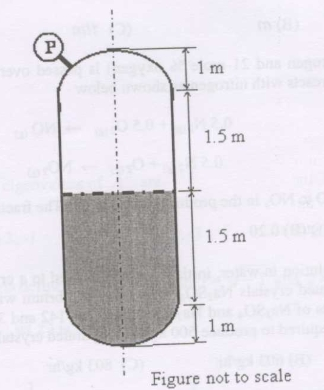
\includegraphics[width=0.25\columnwidth]{figs/qn37.jpg}
\caption{}
\label{fig:qn37.jpg}
\end{figure} 
\hfill{\brak{\text{CH 2008}}}
\begin{enumerate}
\begin{multicols}{2}
    \item $F = 83.6$ ; $P = 64.5$
    \item $F = 83.6$ ; $P = 165.8$
    \item $F = 125.7$ ; $P = 64.5$
    \item $F = 125.7$ ; $P = 165.8$
\end{multicols}
\end{enumerate}

\item A pump draws oil (specific gravity $0.8$) from a storage tank and discharges it to an overhead tank.  
The mechanical energy delivered by the pump to the fluid is $50 \ \text{J/kg}$.  
The velocities at the suction and the discharge points of the pump are $1 \ \text{m/s}$ and $7 \ \text{m/s}$, respectively.  
Neglecting friction losses and assuming kinetic energy correction factor to be unity, the pressure developed by the pump (in kN/m$^2$) is 
\hfill{\brak{\text{CH 2008}}}
\begin{enumerate}
\begin{multicols}{4}
    \item $19.2$
    \item $20.8$
    \item $40$
    \item $80$
\end{multicols}
\end{enumerate}

\item Match the following:  

\begin{tabular}{ll}
\textbf{Group 1} & \textbf{Group 2} \\
(P) Euler number & (1) Viscous force / Inertial force \\
(Q) Froude number & (2) Pressure force / Inertial force \\
(R) Weber number & (3) Inertial force / Gravitational force \\
& (4) Inertial force / Surface tension force
\end{tabular}
\hfill{\brak{\text{CH 2008}}}
\begin{enumerate}
\begin{multicols}{2}
    \item[(A)] $F = 83.6 \, ; \, P = 64.5$
    \item[(B)] $F = 83.6 \, ; \, P = 165.8$
    \item[(C)] $F = 125.7 \, ; \, P = 64.5$
    \item[(D)] $F = 125.7 \, ; \, P = 165.8$
\end{multicols}
\end{enumerate}

\item A pump draws oil (specific gravity 0.8) from a storage tank and discharges it to an overhead tank. The mechanical energy delivered by the pump to the fluid is $50 \, \text{J/kg}$. The velocities at the suction and the discharge points of the pump are $1 \, \text{m/s}$ and $7 \, \text{m/s}$, respectively. Neglecting friction losses and assuming kinetic energy correction factor to be unity, the pressure developed by the pump (in $\text{kN/m}^2$) is
\hfill{\brak{\text{CH 2008}}}
\begin{enumerate}[label=(\Alph*)]
\begin{multicols}{4}
    \item $19.2$
    \item $20.8$
    \item $40$
    \item $80$
\end{multicols}
\end{enumerate}

\item Match the following:
\begin{tabular}{ll}
\textbf{GROUP 1} & \textbf{GROUP 2} \\
(P) Euler number & (1) Viscous force / Inertial force \\
(Q) Froude number & (2) Pressure force / Inertial force \\
(R) Weber number & (3) Inertial force / Gravitational force \\
& (4) Inertial force / Surface tension force \\
\end{tabular}
\hfill{\brak{\text{CH 2008}}}
\begin{enumerate}[label=(\Alph*)]
\begin{multicols}{2}
    \item P-1, Q-2, R-3
    \item P-2, Q-3, R-4
    \item P-3, Q-2, R-1
    \item P-4, Q-3, R-2
\end{multicols}
\end{enumerate}

\item A steady flow field of an incompressible fluid is given by $\vec{V} = (Ax + By) \hat{i} - Ay \hat{j}$, where $A = 1 \, \text{s}^{-1}$, $B = 1 \, \text{s}^{-1}$, and $x, y$ are in meters. The magnitude of the acceleration (in $\text{m/s}^2$) of a fluid particle at $(1, 2)$ is
\hfill{\brak{\text{CH 2008}}}
\begin{enumerate}[label=(\Alph*)]
\begin{multicols}{4}
    \item $1$
    \item $\sqrt{2}$
    \item $\sqrt{5}$
    \item $\sqrt{10}$
\end{multicols}
\end{enumerate}

\item Two identically sized spherical particles $A$ and $B$ having densities $\rho_A$ and $\rho_B$, respectively, are settling in a fluid of density $\rho$. Assuming free settling under turbulent flow conditions, the ratio of the terminal settling velocity of particle $A$ to that of particle $B$ is given by
\begin{figure}[H]
\centering
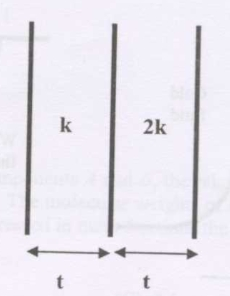
\includegraphics[width=0.25\columnwidth]{figs/qn43.jpg}
\caption{}
\label{fig:qn43.jpg}
\end{figure}
\hfill{\brak{\text{CH 2008}}}
\begin{enumerate}[label=(\Alph*)]
\begin{multicols}{4}
    \item $\sqrt{\frac{(\rho_A - \rho)}{(\rho_B - \rho)}}$
    \item $\sqrt{\frac{(\rho_B - \rho)}{(\rho_A - \rho)}}$
    \item $\frac{(\rho_A - \rho)}{(\rho_B - \rho)}$
    \item $\frac{(\rho_B - \rho)}{(\rho_A - \rho)}$
\end{multicols}\end{enumerate}

\item Consider the scale-up of a cylindrical baffled vessel configured to have the standard geometry (i.e. Height = Diameter). In order to maintain an equal rate of mass transfer under turbulent conditions for a Newtonian fluid, the ratio of the agitator speeds should be \\
(Given $N_1, D_1$ are agitator speed and vessel diameter before scale-up; $N_2, D_2$ are agitator speed and vessel diameter after scale-up)
\hfill{\brak{\text{CH 2008}}}
\begin{enumerate}[label=(\Alph*)]
\begin{multicols}{4}
    \item $\frac{N_1}{N_2} = \frac{D_1}{D_2}$
    \item $\frac{N_1}{N_2} = \frac{D_2}{D_1}$
    \item $\frac{N_1}{N_2} = \left( \frac{D_1}{D_2} \right)^{\frac{2}{3}}$
    \item $\frac{N_1}{N_2} = \left( \frac{D_2}{D_1} \right)^{\frac{2}{3}}$
\end{multicols}
\end{enumerate}

\item Two plates of equal thickness ($t$) and cross-sectional area, are joined together to form a composite as shown in the figure. If the thermal conductivities of the plates are $k$ and $2k$ then the effective thermal conductivity of the composite is
\hfill{\brak{\text{CH 2008}}}
\begin{enumerate}[label=(\Alph*)]
\begin{multicols}{4}
    \item $3k/2$
    \item $4k/3$
    \item $3k/4$
    \item $2k/3$
    \end{multicols}
\end{enumerate}

\item The temperature profile for heat transfer from one fluid to another seperated by a solid wall is
\hfill{\brak{\text{CH 2008}}}
\begin{figure}[H]
    \centering
    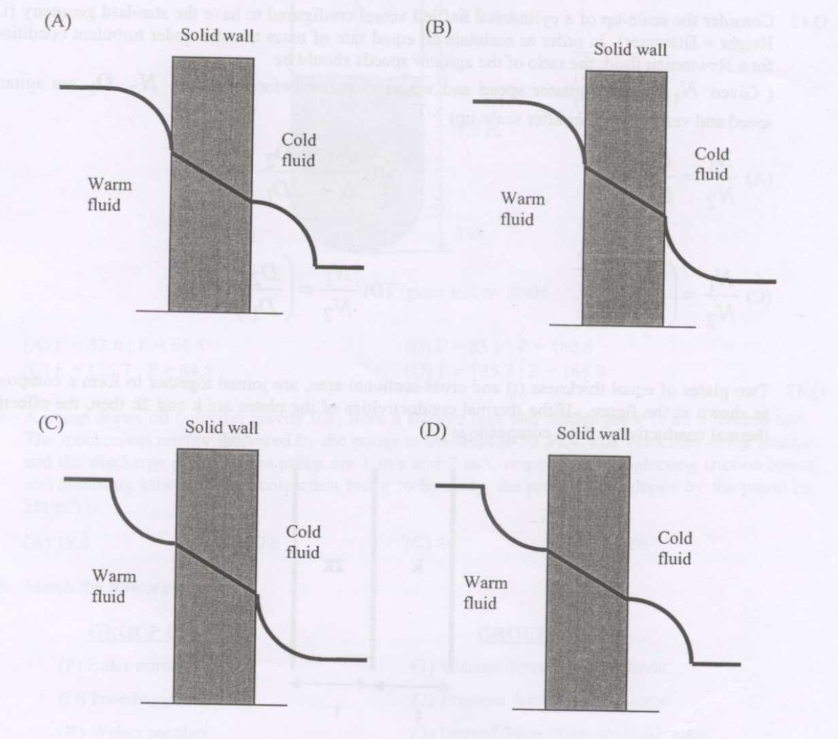
\includegraphics[width=0.5\columnwidth]{figs/qn46.jpg}
    \caption{}
    \label{fig:qn46.jpg}
\end{figure}

\item A rectangular slab of thickness $2b$ along the $x$ axis and extending to infinity along the other directions is initially at concentration $c_{A0}$. At time $t=0$, both surfaces of the slab ($x = \pm b$) have their concentrations increased to $c_{AW}$ and maintained at that value. Solute A diffuses into the solid. The dimensionless concentration $C$ is defined as

\[C = \frac{c_A - c_{A0}}{c_{AW} - c_{A0}}\]

The diffusivity of A inside the solid is assumed constant. At a certain time instant, which ONE of the following is the correct representation of the concentration profile?
\hfill{\brak{\text{CH 2008}}}
\begin{figure}[H]
    \centering
    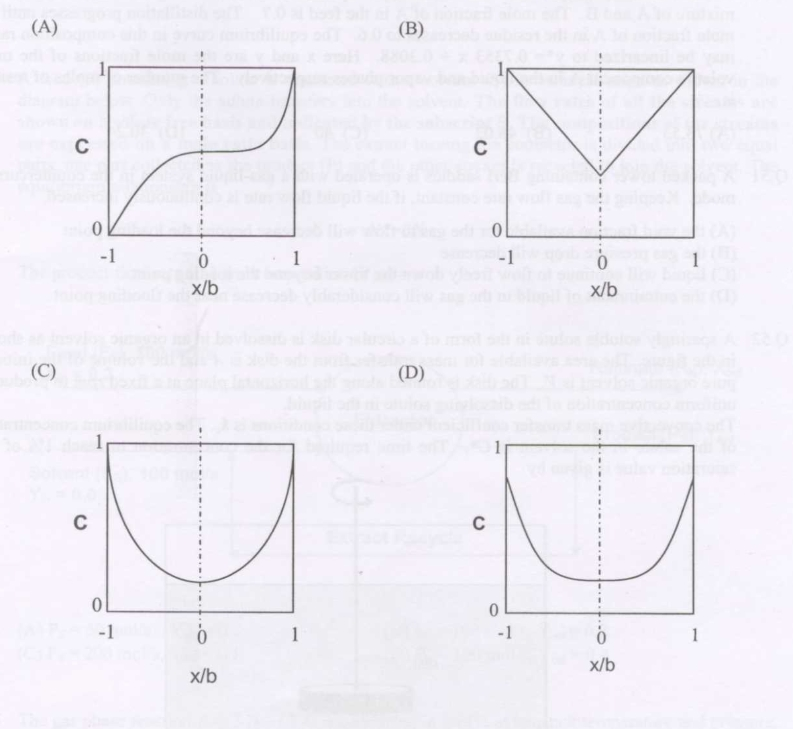
\includegraphics[width=0.5\columnwidth]{figs/qn47.jpg}
    \caption{}
    \label{fig:qn47.jpg}
\end{figure}

\item In a binary mixture containing components $A$ and $B$, the relative volatility of $A$ with respect to $B$ is $2.5$ when mole fractions are used. The molecular weights of $A$ and $B$ are $78$ and $92$ respectively. If the compositions are however expressed in mass fractions the relative volatility will then be
\hfill{\brak{\text{CH 2008}}}
\begin{enumerate}
\begin{multicols}{4}
\item $1.18$
\item $2.12$
\item $2.5$
\item $2.95$
\end{multicols}
\end{enumerate}

\item An ideal flash vaporization is carried out with a binary mixture at constant temperature and pressure. A process upset leads to an increase in the mole fraction of the heavy component in the feed. The flash vessel continues to operate at the previous temperature and pressure and still produces liquid and vapor. After steady state is re-established,
\hfill{\brak{\text{CH 2008}}}
\begin{enumerate}
\item the amount of vapor produced will increase
\item the amount of liquid produced will decrease
\item the new equilibrium compositions of the vapor and liquid products will be different
\item the new equilibrium compositions of the vapor and liquid products will remain as they were before the upset occurred
\end{enumerate}

\item A batch distillation operation is carried out to separate a feed containing $100$ moles of a binary mixture of A and B. The mole fraction of $A$ in the feed is $0.7$. The distillation progresses until mole fraction of A in the residue decreases to $0.6$. The equilibrium curve in this composition range may be linearized to $y^* = 0.7353 \, x + 0.3088$. Here $x$ and $y$ are the mole fractions of the more volatile component A in the liquid and vapor phases respectively. The number of moles of residue is
\hfill{\brak{\text{CH 2008}}}
\begin{enumerate}
\begin{multicols}{4}
\item $73.53$
\item $48.02$
\item $40$
\item $30.24$
\end{multicols}
\end{enumerate}

\item A packed tower containing Berl saddles is operated with a gas-liquid system in the countercurrent mode. Keeping the gas flow rate constant, if the liquid flow rate is continuously increased,
\hfill{\brak{\text{CH 2008}}}
\begin{enumerate}
\item the void fraction available for the gas to flow will decrease
\item the gas pressure drop will decrease
\item liquid will continue to flow freely down the tower beyond the loading point
\item the entrainment of liquid in the gas will considerably decrease near the flooding point
\end{enumerate}

\item A sparingly soluble solute in the form of a circular disk is dissolved in an organic solvent as shown in the figure. The area available for mass transfer from the disk is $A$ and the volume of the initially pure organic solvent is $V$. The disk is rotated along the horizontal plane at a fixed $rpm$ to produce a uniform concentration of the dissolving solute in the liquid.

The convective mass transfer coefficient under these conditions is $k_c$. The equilibrium concentration of the solute in the solvent is $C^*$. The time required for the concentration to reach $1\%$ of the saturation value is given by
\begin{figure}[H]
    \centering
    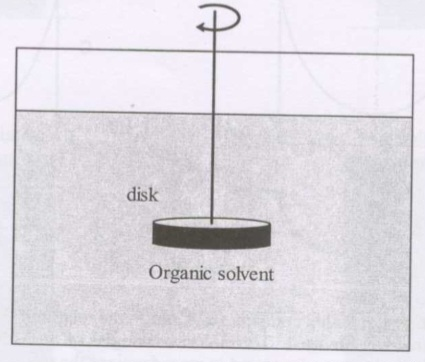
\includegraphics[width=0.25\columnwidth]{figs/qn52.jpg}
    \caption{}
    \label{fig:qn52.jpg}
\end{figure}
\hfill{\brak{\text{CH 2008}}}
\begin{enumerate}
\begin{multicols}{2}
\item `\exp\left(-\frac{k_c A}{V} t\right) = 0.99`
\item `\exp\left(-\frac{k_c A}{V} t\right) = 0.01`
\item `\frac{V}{A k_c} \exp(-0.99) = t
\item `\frac{V}{A k_c} \exp(0.01) = t`
\end{multicols}
\end{enumerate}

\item Air concentrated with solute P is brought in contact with water.At steady state,the bulk concentrations of P in air and water are 0.3 and 0.02 respectively. The equilibrium equation relating the interface compositions is 
\[y_{P,i} = 0.25 \, x_{P,i}\]
Assume that the mass transfer coefficients $F_G$ and $F_L$ are identical. The gas phase mole fraction of P at the interface ($y_{P,i}$) is
\hfill{\brak{\text{CH 2008}}}
\begin{enumerate}
\begin{multicols}{4}
\item $0.0663$
\item $0.075$
\item $0.16$
\item $0.3$
\end{multicols}
\end{enumerate}

\item A feed (F) containing a solute is contacted with a solvent (S) in an ideal stage as shown in the diagram below. Only the solute transfers into the solvent. The flow rates of all the streams are shown on a solute free basis and indicated by the subscript S. The compositions of the streams are expressed on a mole ratio basis. The extract leaving the contactor is divided into two equal parts, one part collected as the product (P) and the other stream is recycled to join the solvent. The equilibrium relationship is
\[Y^* = 2X\]
The product flow rate ($P_S$) and composition ($Y_{out}$) are
\begin{figure}[H]
    \centering
    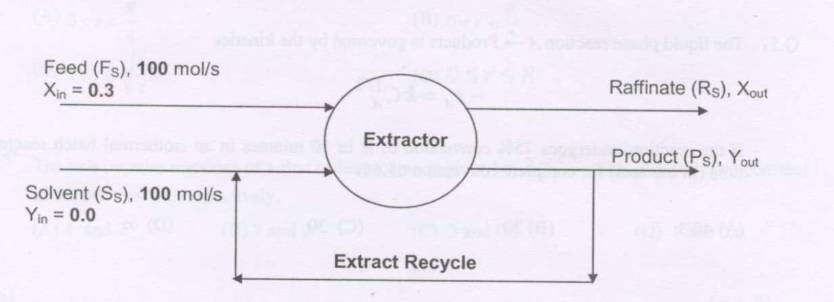
\includegraphics[width=0.25\columnwidth]{figs/qn54.jpg}
    \caption{}
    \label{fig:qn54.jpg}
\end{figure}
\hfill{\brak{\text{CH 2008}}}
\begin{enumerate}
\begin{multicols}{2}
\item P_S = 50 \, \text{mol/s}, \quad Y_{\text{out}} = 0.3 
\item P_S = 100 \, \text{mol/s}, \quad Y_{\text{out}} = 0.2 
\item  P_S = 200 \, \text{mol/s}, \quad Y_{\text{out}} = 0.1 
\item P_S = 100 \, \text{mol/s}, \quad Y_{\text{out}} = 0.4 
\end{multicols}
\end{enumerate}

\item The gas phase reaction $\mathrm{A + 3B \rightarrow 2C}$ is conducted in a PFR at constant temperature and pressure. The PFR achieves a conversion of $20\%$ of A. The feed is a mixture of A, B and an inert I. It is found that the concentration of A remains the same throughout the reactor. \\
Which \textbf{ONE} of the following ratios of inlet molar rates ($F_{A,in}: F_{B,in}: F_{I,in}$) is consistent with this observation? Assume the reaction mixture is an ideal gas mixture.
\hfill{\brak{\text{CH 2008}}}
\begin{enumerate}
\begin{multicols}{4}
\item $2:3:0$
\item $2:2:1$
\item $3:2:1$
\item $1:2:1$
\end{multicols}
\end{enumerate}

\item The elementary liquid phase series-parallel reaction scheme
\[\begin{aligned}A &\rightarrow B \rightarrow C \\A &\rightarrow R\end{aligned}\]
is to be carried out in an isothermal CSTR. The rate laws are given by
\[\begin{aligned}r_R &= k' C_A \\r_B &= k C_A - k C_B\end{aligned}\]
Feed is pure A. The space time of the CSTR which results in the maximum exit concentration of B is given by
\hfill{\brak{\text{CH 2008}}}
\begin{enumerate}
\begin{multicols}{2}
\item $\frac{1}{\sqrt{k k'}}$
\item $\frac{1}{\sqrt{k'(k + k')}}$
\item $\frac{1}{(k + k')}$
\item $\frac{1}{\sqrt{k(k + k')}}$
\end{multicols}
\end{enumerate}

\item  The liquid phase reaction $A \rightarrow$ Products is governed by the kinetics
\[-r_A = k C_A^{1/2}\]
If the reaction undergoes $75\%$ conversion of $A$ in 10 minutes in an isothermal batch reactor, the time (in minutes) for complete conversion of $A$ is
\hfill{\brak{\text{CH 2008}}}
\begin{enumerate}
\begin{multicols}{4}
\item $40/3$
\item $20$
\item $30$
\item $\infty$
\end{multicols}
\end{enumerate}

\item The homogeneous reaction $\mathrm{A + B \rightarrow C}$ is conducted in an adiabatic CSTR at $800 \, \mathrm{K}$ so as to achieve a $30\%$ conversion of A. The relevant specific heats and enthalpy change of reaction are given by
\[\begin{aligned}C_{P,A} &= 100 \, \mathrm{J/(mol \, K)}, \, C_{P,C} = 150 \, \mathrm{J/(mol \, K)} \\C_{P,B} &= 50 \, \mathrm{J/(mol \, K)}, \, \Delta H^{rxn} = -100 \, \mathrm{kJ/mol}\end{aligned}\]
If the feed, a mixture of A and B, is available at $550 \, \mathrm{K}$, the mole fraction of A in the feed that is consistent with the above data is
\hfill{\brak{\text{CH 2008}}}
\begin{enumerate}
\begin{multicols}{4}
\item $5/7$
\item $1/4$
\item $1/2$
\item $2/7$
\end{multicols}
\end{enumerate}

\item The irreversible zero order reaction $A \rightarrow B$ takes place in a porous cylindrical catalyst that is sealed at both ends as shown in the figure. Assume dilute concentrations and neglect any variations in the axial direction.
\begin{figure}[H]
    \centering
    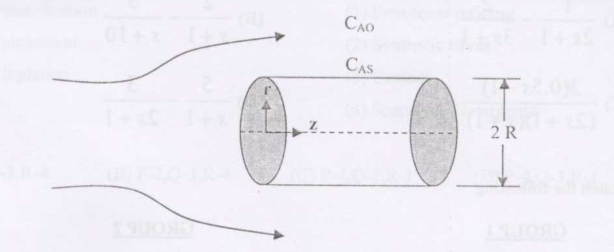
\includegraphics[width=0.25\columnwidth]{figs/qn59.jpg}
    \caption{}
    \label{fig:qn.59.jpg}
\end{figure}
The steady state concentration profile is
\[\frac{C_A}{C_{AS}} = 1 + \frac{\phi_o^2}{4} \left[ \left( \frac{r}{R} \right)^2 - 1 \right]\]
where $\phi_o$ is the Thiele modulus. For $\phi_o = 4$, the range of $r$ where $C_A=0$ is
\hfill{\brak{\text{CH 2008}}}
\begin{enumerate}
\begin{multicols}{2}
\item $0 < r < \frac{R}{4}$
\item $0 < r < \frac{R}{2}$
\item $0 \leq r \leq \sqrt{\frac{3}{4}} R$
\item $0 \leq r \leq R$
\end{multicols}
\end{enumerate}

\item The unit impulse response of a first order process is given by $2 e^{-0.5 t}$. The gain and time constant of the process are, respectively,
\hfill{\brak{\text{CH 2008}}}
\begin{enumerate}
\begin{multicols}{4}
    \item $4$ and $2$
    \item $2$ and $2$
    \item $2$ and $0.5$
    \item $1$ and $0.5$
\end{multicols}
\end{enumerate}

\item A unit step input is given to a process that is represented by the transfer function $\frac{(s+2)}{(s+5)}$. The initial value ($t = 0^+$) of the response of the process to the step input is
\hfill{\brak{\text{CH 2008}}}
\begin{enumerate}
\begin{multicols}{4}
    \item $0$
    \item $2/5$
    \item $1$
    \item $\infty$
\end{multicols}
\end{enumerate}

\item A tank of volume $0.25 \, \text{m}^3$ and height $1 \, \text{m}$ has water flowing in at $0.05 \, \text{m}^3/\text{min}$. The outlet flow rate is governed by the relation
\[F_{out} = 0.1 \, h\]
where $h$ is the height of the water in the tank in m and $F_{out}$ is the outlet flow rate in $\text{m}^3/\text{min}$.

The inlet flow rate changes suddenly from its nominal value of $0.05 \, \text{m}^3/\text{min}$ to $0.15 \, \text{m}^3/\text{min}$ and remains there. The time (in minutes) at which the tank will begin to overflow is given by
\hfill{\brak{\text{CH 2008}}}
\begin{enumerate}
\begin{multicols}{4}
    \item $0.28$
    \item $1.01$
    \item $1.73$
    \item $\infty$
\end{multicols}    
\end{enumerate}

\item Which ONE of the following transfer functions corresponds to an inverse response process with a positive gain?
\hfill{\brak{\text{CH 2008}}}
\begin{enumerate}
\begin{multicols}{2}
    \item $\frac{1}{2s+1} - \frac{2}{3s+1}$
    \item $\frac{2}{s+1} - \frac{5}{s+10}$
    \item $\frac{3(0.5s-1)}{(2s+1)(s+1)}$
    \item $\frac{5}{s+1} - \frac{3}{2s+1}$
\end{multicols}
\end{enumerate}

\item Match the following
\begin{center}
\begin{tabular}{c|c}
GROUP 1 & GROUP 2 \\
\hline
(P) Temperature & (1) Hot wire anemometry \\
(Q) Pressure & (2) Strain Gauge \\
(R) Flow & (3) Chromatographic analyzer \\
& (4) Pyrometer \\
\end{tabular}
\end{center}
\hfill{\brak{\text{CH 2008}}}
\begin{enumerate}
\begin{multicols}{4}
    \item P-1, Q-2, R-3
    \item P-4, Q-1, R-3
    \item P-1, Q-2, R-4
    \item P-4, Q-2, R-1
\end{multicols}
\end{enumerate}

\item  Match the following
\begin{center}
\begin{tabular}{c|c}
GROUP 1 & GROUP 2 \\
\hline
(P) Ziegler Nichols & (1) Process Reaction Curve \\
(Q) Under damped response & (2) Decay ratio \\
(R) Feed-forward Control & (3) Frequency Response \\
& (4) Disturbance measurement \\
\end{tabular}
\end{center}
\hfill{\brak{\text{CH 2008}}}
\begin{enumerate}
\begin{multicols}{4}
    \item P-3, Q-2, R-4
    \item P-1, Q-2, R-3
    \item P-3, Q-4, R-2
    \item P-1, Q-4, R-2
\end{multicols}
\end{enumerate}

\item A reactor has been installed at a cost of Rs. 50,000 and is expected to have a working life of 10 years with a scrap value of Rs. 10,000. The capitalized cost (in Rs.) of the reactor based on an annual compound interest rate of $5\%$ is
\hfill{\brak{\text{CH 2008}}}
\begin{enumerate}
\begin{multicols}{4}
    \item $1,13,600$
    \item $42,000$
    \item $52,500$
    \item $10,500$
\end{multicols}
\end{enumerate}

\item  In a shell and tube heat exchanger, if the shell length is $L_S$, the baffle spacing is $L_B$ and the thickness of baffle is $t_b$, the number of baffles on the shell side, $\mathrm{N}_b$, is
\hfill{\brak{\text{CH 2008}}}
\begin{enumerate}
\begin{multicols}{4}
    \item $\frac{L_S}{L_B + t_b}$
    \item $\frac{L_S}{L_B} - 1$
    \item $\frac{L_S}{L_B + t_b} + 1$
    \item $\frac{L_S}{L_B + t_b} + 2$
\end{multicols}
\end{enumerate}

\item Match the unit processes in Group 1 with the industries in Group 2
\begin{center}
\begin{tabular}{c|c}
GROUP 1 & GROUP 2 \\
\hline
(P) Saponification & (1) Petroleum refining \\
(Q) Calcination & (2) Synthetic fibres \\
(R) Alkylation & (3) Cement \\
& (4) Soaps and Detergents \\
\end{tabular}
\end{center}
\hfill{\brak{\text{CH 2008}}}
\begin{enumerate}
\begin{multicols}{4}
    \item P-1,Q-3,R-4
    \item P-2,Q-3,R-4
    \item P-4,Q-2,R-1
    \item P-4,Q-3,R-1
\end{multicols}
\end{enumerate}

\item \quad Which ONE of the following process sequences is used in the production of synthesis gas?
\hfill{\brak{\text{CH 2008}}}
\begin{enumerate}
\item Desulphurization $\rightarrow$ Steam reforming $\rightarrow$ Hot K$_2$CO$_3$ cycle 
\item Steam reforming $\rightarrow$ Desulphurization $\rightarrow$ Hot K$_2$CO$_3$ cycle
\item Hot K$_2$CO$_3$ cycle $\rightarrow$ Steam reforming $\rightarrow$ Desulphurization
\item Hot K$_2$CO$_3$ cycle $\rightarrow$ Desulphurization $\rightarrow$ Steam reforming
\end{enumerate}

\item Which ONE of the following process sequences is used in the sugar industry?
\hfill{\brak{\text{CH 2008}}}
\begin{enumerate}
\item Ca$_2$HPO$_4$/ Lime Treatment $\rightarrow$ Crystallization $\rightarrow$ Crushing
\item Ca$_2$HPO$_4$/ Lime Treatment $\rightarrow$ Multiple stage evaporation $\rightarrow$ Crystallization
\item Crushing $\rightarrow$ Crystallization $\rightarrow$ Ca$_2$HPO$_4$/ Lime Treatment
\item Multiple stage evaporation $\rightarrow$ Crystallization $\rightarrow$ Ca$_2$HPO$_4$/ Lime Treatment
\end{enumerate}
\section*{Common Data for Questions 71,72 and 73:}
Methane and steam are fed to a reactor in molar ratio $1:2$. The following reactions take place,
\[\begin{aligned}\mathrm{CH}_4(\mathrm{g}) + 2\mathrm{H}_2\mathrm{O}(\mathrm{g}) &\rightarrow \mathrm{CO}_2(\mathrm{g}) + 4\mathrm{H}_2(\mathrm{g}) \\\mathrm{CH}_4(\mathrm{g}) + \mathrm{H}_2\mathrm{O}(\mathrm{g}) &\rightarrow \mathrm{CO}(\mathrm{g}) + 3\mathrm{H}_2(\mathrm{g})\end{aligned}\]
where $\mathrm{CO}_2$ is the desired product, $\mathrm{CO}$ is the undesired product and $\mathrm{H}_2$ is a byproduct. The exit stream has the following composition

\begin{tabular}{|c|c|c|c|c|c|}
\hline
Species & $\mathrm{CH}_4$ & $\mathrm{H}_2\mathrm{O}$ & $\mathrm{CO}_2$ & $\mathrm{H}_2$ & $\mathrm{CO}$ 
\hline
Mole \% & 4.35 & 10.88 & 15.21 & 67.39 & 2.17 
\hline
\end{tabular}
\item [\textbf{71)}] The selectivity for desired product relative to undesired product is
\hfill{\brak{\text{CH 2008}}}
\begin{enumerate}
\begin{multicols}{4}
\item $2.3$
\item $3.5$
\item $7$
\item $8$
\end{multicols}
\end{enumerate}

\item [\textbf{72)}] The fractional yield of $\mathrm{CO}_2$ is
(where fractional yield is defined as the ratio of moles of the desired product formed to the moles that would have been formed if there were no side reactions and the limiting reactant had reacted completely)
\hfill{\brak{\text{CH 2008}}}
\begin{enumerate}
\begin{multicols}{4}
\item $0.7$
\item $0.88$
\item $1$
\item $3.5$
\end{multicols}
\end{enumerate}

\item [\textbf{73)}] The fractional conversion of methane is
\hfill{\brak{\text{CH 2008}}}
\begin{enumerate}
\begin{multicols}{4}
\item $0.4$
\item $0.5$
\item $0.7$
\item $0.8$
\end{multicols}
\end{enumerate}

\section*{Common Data for Questions 74 and 75:}
A liquid is flowing through a reactor at a constant flow rate. A step input of tracer at a molar flow rate of $1$ mol/min is given to the reactor at time $t = 0$. The time variation of the concentration ($C$) of the tracer at the exit of the reactor is as shown in the figure:
\begin{enumerate}
\item[\textbf{74)}] The volumetric flow rate of the liquid through the reactor (in L/min) is
\hfill{\brak{\text{CH 2008}}}
\begin{enumerate}
\begin{multicols}{4}
\item $1$
\item $2$
\item $1.5$
\item $4$
\end{multicols}
\end{enumerate}

\item[\textbf{75)}] The mean residence time of the fluid in the reactor (in minutes) is
\hfill{\brak{\text{CH 2008}}}
\begin{enumerate}
\begin{multicols}{4}
\item $1$
\item $2$
\item $3$
\item $4$
\end{multicols}
\end{enumerate}

\section*{Linked Answer Questions: Q.76 to Q.85 carry two marks each}

\subsection*{Statement for Linked Answer Questions 76 and 77:}
A binary mixture containing species 1 and 2 forms an azeotrope at $105.4^\circ$C and $1.013$ bar. The liquid phase mole fraction of component 1 ($x_1$) of this azeotrope is $0.62$. At $105.4^\circ$C, the pure component vapor pressures for species 1 and 2 are $0.878$ bar and $0.665$ bar, respectively. Assume that the vapour phase is an ideal gas mixture. The van Laar constants, $A$ and $B$, are given by the expressions:
\[\begin{aligned}A &= \left[ 1 + \frac{x_2 \ln \gamma_2}{x_1 \ln \gamma_1} \right]^2 \ln \gamma_1, \\B &= \left[ 1 + \frac{x_1 \ln \gamma_1}{x_2 \ln \gamma_2} \right]^2 \ln \gamma_2\end{aligned}\]

    \item[\textbf{76)}] The activity coefficients $(\gamma_1, \gamma_2)$ under these conditions are
    \hfill{\brak{\text{CH 2008}}}
    \begin{enumerate}
    \begin{multicols}{4}
        \item[(A)] $(0.88, 0.66)$
        \item[(B)] $(1.15, 1.52)$
        \item[(C)] $(1.52, 1.15)$
        \item[(D)] $(1.52, 0.88)$
        \end{multicols}
    \end{enumerate}
    \item[\textbf{77)}] The van Laar constants $(A, B)$ are
    \hfill{\brak{\text{CH 2008}}}
    \begin{enumerate}
    \begin{multicols}{4}
        \item[(A)] $(0.92, 0.87)$
        \item[(B)] $(1.00, 1.21)$
        \item[(C)] $(1.12, 1.00)$
        \item[(D)] $(1.52, 1.15)$
    \end{multicols}
    \end{enumerate}

\subsection*{Statement for Linked Answer Questions 78 and 79:}
A siphon tube having a diameter of $2$ cm draws water from a large open reservoir and discharges into the open atmosphere as shown in the figure. Assume incompressible fluid and neglect frictional losses. \quad $(g = 9.8 \, \text{m/s}^2)$

\begin{figure}[H]
    \centering
    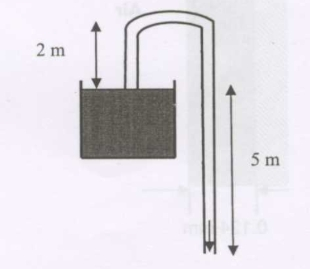
\includegraphics[width=0.25\columnwidth]{figs/qn 78.jpg}
    \caption{}
    \label{fig:qn77.jpg}
\end{figure}

    \item[\textbf{78)}] The velocity (in m/s) at the discharge point is
    \hfill{\brak{\text{CH 2008}}}
    \begin{enumerate}
    \begin{multicols}{4}
        \item[(A)] $9.9$
        \item[(B)] $11.7$
        \item[(C)] $98$
        \item[(D)] $136.9$
        \end{multicols}
    \end{enumerate}
    \item[\textbf{79)}] The volumetric flow rate (in L/s) of water at the discharge is
    \hfill{\brak{\text{CH 2008}}}
    \begin{enumerate}
    \begin{multicols}{4}
        \item $3.11$
        \item $3.67$
        \item $30.77$
        \item $42.99$
        \end{multicols}
    \end{enumerate}
    \section*{Statement for Linked Answer Questions 80 \& 81:}
The liquid phase reaction $A \rightarrow$ Products is to be carried out at constant temperature in a CSTR followed by a PFR in series. The overall conversion of $A$ achieved by the reactor system (CSTR + PFR) is $95\%$. The CSTR has a volume of 75 liters. Pure $A$ is fed to the CSTR at a concentration $C_{A0} = 2$ mol/liter and a volumetric flow rate of 4 liters/min. The kinetics of the reaction is given by
\[-r_A = 0.1 \, C_A^2 \quad \frac{\text{mol}}{\text{liter} \cdot \text{min}}\]

    \item[\textbf{80)}] The conversion achieved by the CSTR is
    \hfill{\brak{\text{CH 2008}}}
    \begin{enumerate}
    \begin{multicols}{4}
        \item[(A)] $40\%$
        \item[(B)] $50\%$
        \item[(C)] $60\%$
        \item[(D)] $80\%$
        \end{multicols}
    \end{enumerate}
    \item[\textbf{81)}] The volume of the PFR required (in liters) is
    \hfill{\brak{\text{CH 2008}}}
    \begin{enumerate}
    \begin{multicols}{4}
        \item[(A)] $380$
        \item[(B)] $350$
        \item[(C)] $75$
        \item[(D)] $35$
        \end{multicols}
    \end{enumerate}
    \section*{Statement for Linked Answer Questions 82 and 83:}
A thin liquid film flows at steady state along a vertical surface as shown in the figure. The average velocity of the liquid film is $0.05$ m/s. The viscosity of the liquid is $1$ cP and its density is $1000$ kg/m$^3$. The initially pure liquid absorbs a sparingly soluble gas from air as it flows down. The length of the wall is $2$ m and its width is $0.5$ m. The solubility of the gas in the liquid is $3.4 \times 10^{-2}$ kmol/m$^3$ and isothermal conditions may be assumed.

\begin{figure}[H]
    \centering
    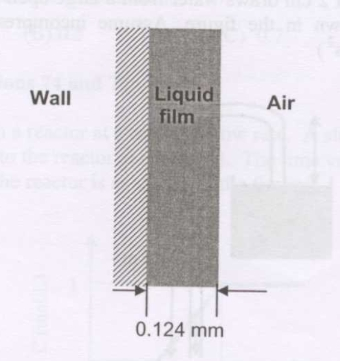
\includegraphics[width=0.25\columnwidth]{figs/qn 82.jpg}
    \caption{}
    \label{fig:qn81.jpg}
\end{figure}

    \item[\textbf{82)}] If the exit average concentration in the liquid is measured to be $1.4 \times 10^{-2}$ kmol/m$^3$, the total mass transfer rate (in kmol/s) of the sparingly soluble gas into the liquid is
    \hfill{\brak{\text{CH 2008}}}
    \begin{enumerate}
    \begin{multicols}{4}
        \item[(A)] $0.133 \times 10^{-4}$
        \item[(B)] $0.434 \times 10^{-7}$
        \item[(C)] $3.4 \times 10^{-2}$
        \item[(D)] $17 \times 10^{-2}$
    \end{multicols}
    \end{enumerate}
 \item[\textbf{83)}] The mass transfer coefficient $k_{c,\text{avg}}$ (in m/s), averaged along the length of the vertical surface is
 \hfill{\bracc,cck{\text{CH 2008}}}
    \begin{enumerate}
    \begin{multicols}{4}
        \item[(A)] $2.94 \times 10^{-6}$
        \item[(B)] $2.27 \times 10^{-6}$
        \item[(C)] $1.94 \times 10^{-6}$
        \item[(D)] $1.65 \times 10^{-6}$
    \end{multicols}
    \end{enumerate}
\section*{Statement for Linked Answer Questions 84 and 85:}
The cross-over frequency associated with a feedback loop employing a proportional controller to control the process represented by the transfer function
\[G_p(s) = \frac{2 e^{-s}}{(\tau s + 1)^2}, \quad \text{(units of time is minutes)}\]
is found to be $0.6$ rad/min. Assume that the measurement and valve transfer functions are unity.

    \item[\textbf{84)}] The time constant, $\tau$ (in minutes) is
    \hfill{\brak{\text{CH 2008}}}
    \begin{enumerate}
    \begin{multicols}{4}
        \item[(A)] $1.14$
        \item[(B)] $1.92$
        \item[(C)] $3.23$
        \item[(D)] $5.39$
        \end{multicols}
    \end{enumerate}
    \item[\textbf{85)}] If the control loop is to operate at a gain margin of $2.0$, the gain of the proportional controller must equal
    \hfill{\brak{\text{CH 2008}}}
    \begin{enumerate}
    \begin{multicols}{4}
        \item[(A)] $0.85$
        \item[(B)] $2.87$
        \item[(C)] $3.39$
        \item[(D)] $11.50$
    \end{multicols}
    \end{enumerate}
\centering
\textbf{END OF THE QUESTION PAPER}


\end{enumerate}
\end{document}



































































































